\chapter{Dataset description}
\label{ch:dataset_description_neo4j}%
The main dataset used can be downloaded from the site \href{https://www.aminer.org/citation}{www.aminer.org}, in particular, the latest version of data was employed, namely DBLP-Citation network V13.
The dataset was not entirely imported in Neo4j because it was huge and our machines with limited computing power were not able to handle it, so just a part of it was taken, containing information about 2315 papers.

The following table shows the dataset's fields that were used, associated with their respective meaning, name, and role in the created database.
The fields publisher and location were not present in the original dataset, that's why we created this information from scratch, but this aspect is further discussed in the following chapter.
\begin{table}[H]
    \centering
    \begin{tabular}{| c | c | c | c | c |}
        \hline
        \textbf{Field name} & \textbf{Type} & \textbf{Description} & \textbf{Name in Neo4j} & \textbf{Usage in Neo4j}  \T\B \\
        \hline
        \hline
        \_id                & String        & paper ID             & id                     & node Paper\T\B              \\
        title               & String        & paper title          & title                  & node Paper\T\B              \\
        year                & Integer       & paper year           & year                   & node Paper\T\B              \\
        lang                & String        & paper language       & lang                   & node Paper\T\B              \\
        doi                 & String        & paper DOI            & doi                    & node Paper\T\B              \\
        url                 & String        & paper URL            & url                    & node Paper\T\B              \\
        abstract            & String        & paper abstract       & abstract               & node Paper \T\B             \\
        keywords[i]         & String        & paper keyword        & keyword                & node Keyword\T\B            \\
        fos[i]              & String        & paper field of study & fos                    & node Fos\T\B                \\
        references[i]       & String        & paper reference      & REFERENCES             & relation REFERENCES\T\B     \\
        page\_start         & Integer       & start page           & page\_start            & attribute IS\_PART\_OF \T\B \\
        page\_end           & Integer       & end page             & page\_end              & attribute IS\_PART\_OF \T\B \\
        authors.\_id        & String        & author ID            & id                     & node Author\T\B             \\
        authors.name        & String        & author name          & name                   & node Author\T\B             \\
        authors.org         & String        & author affiliation   & affiliation            & attribute WRITES\T\B        \\
        venue.raw           & String        & publication name     & name                   & node Publication \T\B       \\
        isbn                & String        & book ISBN            & isbn                   & node Book \T\B              \\
        publisher           & String        & publisher name       & publisher              & node Book/Journal \T\B      \\
        issn                & String        & journal ISSN         & issn                   & node Journal \T\B           \\
        volume              & String        & journal volume       & volume                 & node Journal \T\B           \\
        issue               & String        & journal issue        & issue                  & node Journal \T\B           \\
        location            & String        & conference location  & location               & node Conference \T\B        \\
        \hline
    \end{tabular}
    \\[8pt]
    \caption{Description of the data used in the project and relationship between original dataset and imported data.}
    \label{tab:dataset_description}%
\end{table}


\chapter{Data upload}
\label{ch:data_upload_neo4j}%


\section{Pre-processing}
\label{sec:pre_processing_neo4j}%
Before uploading the data in Neo4j, the dataset was downloaded from the website mentioned above, and just a part of it has been extracted.
Then some ad-hoc Python scripts have been used to do a first-level cleaning of the data since we found some inconsistency in it.
Specifically, the cleaning involved the following aspects:
\begin{itemize}
    \item Some numerical attributes were wrapped in NumberInt(\ldots) string.
    This is not a standard way to store numeric values in JSON so it couldn't be parsed by the Neo4j JSON parser.
    We unwrapped all numeric values stored this way, leaving only the actual value;
    \item Some of the ISSN attributes did not conform to the standard and correct pattern, so the wrong ones have been eliminated;
\end{itemize}
After that, to distinguish the type of publication, a Python script was made to infer it based on the attributes of the paper: if it has an ISBN is a Book, if it has an ISSN, volume or issue is a Journal otherwise it is a Conference.

To have a more complete domain it has been decided to add the fields publisher to Book and Journal, and location to Conference.
These values were taken from the web and added randomly to the papers using a Python script.

Lastly, since just a subset of the dataset has been used, there were very few connections among the nodes, so, thanks to other Python scripts, some values were added randomly to the fields keyword, fos, and references of each paper such that the graph is more connected and more meaningful queries can be performed.


\section{Upload process}
\label{sec:upload_process_neo4j}%
The JSON file called \verb|dataset.json| was used to upload the data, it was put in the \verb|import| folder of Neo4j, and then with the following commands, the data were imported using cypher-shell.

To be sure that at the beginning the database is empty, all possible parameters, nodes, and relationships are deleted with this command.
\begin{lstlisting}[label={lst:upload_process1}]
:params {};
MATCH(n) DETACH DELETE n;
\end{lstlisting}
To use the importing commands it is first necessary to install the \verb|apoc| library and emulate the following steps to be able to use the \verb|apoc.load.json| with which we read the dataset file.
For security reasons, procedures that use internal APIs are disabled by default.
They can be enabled by specifying config in \verb|NEO4J_HOME/conf/neo4j.conf| e.g. \verb|dbms.security.|\verb|procedures.unrestricted=apoc.*|.

You can also whitelist procedures and functions, in general, to be loaded using
\begin{center}
    \verb|dbms.security.procedures.whitelist=apoc.coll.*,apoc.load.*|
\end{center}
We are particularly interested in the last one.
\begin{enumerate}
    \item\textbf{Create Paper nodes with their attributes, create Fos and Keyword nodes} \\
    The following command creates all nodes with label \verb|Paper|, setting the attributes \verb|id|, \verb|title|, \verb|year|, \verb|lang|, \verb|doi|, \verb|url|, \verb|abstract|; then it creates the nodes with label \verb|Keyword| requiring that the value is not null, moreover \verb|Paper| and \verb|Keyword| are linked with the relationship \verb|HIGHLIGHTS|.
    The same thing is done for \verb|Fos| nodes, that are linked with \verb|Paper| nodes through \verb|BELONGS_TO| relationship.
    \begin{lstlisting}[label={lst:upload_process2}]
CAll apoc.load.json('dataset.json') YIELD value
CREATE (p:Paper {id:value._id, title:value.title, year:value.year, lang:value.lang, doi:value.doi, url:value.url, abstract:value.abstract})
WITH p, value
UNWIND value.keywords AS kw
WITH p, value, kw WHERE kw IS NOT NULL
MERGE (k:Keyword {keyword:kw})
MERGE (p)-[h:HIGHLIGHTS]->(k)
WITH p, value
UNWIND value.fos AS fos
WITH p, value, fos WHERE fos IS NOT NULL
MATCH (p:Paper {id:value._id})
MERGE (f:Fos {fos:fos})
MERGE (p)-[b:BELONGS_TO]->(f)
    \end{lstlisting}
    \item \textbf{Create Author nodes and the relationship WRITES} \\
    The following command creates all nodes with label \verb|Author| requiring that \verb|id| and \verb|name| attributes are not null.
    Next, all \verb|Author| nodes are linked with their \verb|Paper| nodes using the \verb|WRITES| relationship, assigning the property \verb|affiliation| when this information is present.
    \begin{lstlisting}[label={lst:author_writes}]
CALL apoc.load.json('dataset.json') YIELD value
UNWIND value.authors AS aut
WITH aut, value
WHERE aut._id IS NOT NULL AND aut.name IS NOT NULL
MERGE (a:Author {id:aut._id, name:aut.name})
WITH a, aut, value
MATCH (p:Paper {id:value._id})
CREATE (a)-[w:WRITES {affiliation:aut.org}]->(p)
    \end{lstlisting}
    \item \textbf{Create Book nodes} \\
    The nodes with label \verb|Book| are created, setting also the label \verb|Publication|, and these entities have the attributes \verb|name| and \verb|publisher|.
    The command also links \verb|Paper| nodes to \verb|Book| nodes using the \verb|IS_PART_OF| relationship, adding to it the properties \verb|page_start| and \verb|page_end|.
    We also allow these attributes to be null, so we don't check their presence when adding them, because in graph databases we can have heterogeneous nodes' structures without any problem and this permits us to explore the peculiarity and strength of this technology.
    \begin{lstlisting}[label={lst:book}]
CALL apoc.load.json('dataset.json') YIELD value
UNWIND value.venue AS ven
WITH value, ven
WHERE value.publication_type = "Book"
CREATE (b:Publication:Book {isbn:value.isbn, publisher:value.publisher, name:ven.raw})
WITH b, value
MATCH (p:Paper {id:value._id})
CREATE (p)-[i:IS_PART_OF {page_start:toInteger(value.page_start), page_end:toInteger(value.page_end)}]->(b)
    \end{lstlisting}
    \item \textbf{Create Conference nodes} \\
    The nodes with label \verb|Conference| are created, setting also the label \verb|Publication|, and \verb|name| and \verb|location| attributes of the conference.
    Then \verb|Paper| nodes are linked with \verb|Conference| nodes using the \verb|IS_PART_OF| relationship setting the properties \verb|page_start| and \verb|page_end|.
    \begin{lstlisting}[label={lst:conference}]
CALL apoc.load.json('dataset.json') YIELD value
UNWIND value.venue AS ven
WITH value, ven
WHERE value.publication_type = "Conference"
CREATE (c:Publication:Conference {name:ven.raw, location:value.location})
WITH c, value
MATCH (p:Paper {id:value._id})
CREATE (p)-[i:IS_PART_OF {page_start:toInteger(value.page_start), page_end:toInteger(value.page_end)}]->(c)
    \end{lstlisting}
    \item \textbf{Create Journal nodes} \\
    The nodes with label \verb|Journal| are created, setting also the label \verb|Publication| and its properties \verb|name|, \verb|publisher|, \verb|issn|, \verb|volume| and \verb|issue|.
    Then \verb|Paper| nodes are linked with \verb|Journal| nodes using the \verb|IS_PART_OF| relationship setting the properties \verb|page_start| and \verb|page_end|.
    \begin{lstlisting}[label={lst:journal}]
CALL apoc.load.json('dataset.json') YIELD value
UNWIND value.venue AS ven
WITH value, ven
WHERE value.publication_type = "Journal"
CREATE (j:Publication:Journal {issn:value.issn, publisher:value.publisher, name:ven.raw, volume:value.volume, issue:value.issue})
WITH j, value
MATCH (p:Paper {id:value._id})
CREATE (p)-[i:IS_PART_OF {page_start:toInteger(value.page_start), page_end:toInteger(value.page_end)}]->(j)
    \end{lstlisting}
    \item \textbf{Create REFERENCES relationship} \\
    With the following command, the \verb|REFERENCES| relationship between \verb|Paper| nodes are created.
    \begin{lstlisting}[label={lst:references}]
CALL apoc.load.json('dataset.json') YIELD value
UNWIND value.references AS ref
WITH value,ref
WHERE ref IS NOT NULL
MATCH (a:Paper {id:value._id})
MATCH (b:Paper {id:ref})
MERGE (a)-[r:REFERENCES]->(b)
    \end{lstlisting}
\end{enumerate}
\begin{table}[H]
    \begin{center}
        \begin{tabular}{| c | c |}
            \hline
            \textbf{Label} & \textbf{Quantity}  \T\B \\
            \hline
            \hline
            Paper          & 2315\T\B              \\
            Author         & 3546\T\B              \\
            Fos            & 155\T\B               \\
            Keyword        & 4343\T\B              \\
            Book           & 372\T\B               \\
            Conference     & 612\T\B               \\
            Journal        & 1315\T\B              \\
            \hline
            \hline
            \textbf{Total} & 12658\T\B             \\
            \hline
        \end{tabular}
        \\[8pt]
        \caption{Summary with node quantity for each label.}
        \label{tab:upload_process}%
    \end{center}
\end{table}


\chapter{Graph diagram}
\label{ch:graph_diagram_neo4j}%
In the realization process from the ER model to the graph diagram, some changes have been made to better exploit the features of Neo4j, prioritizing connections between data.
For this reason nodes with the following labels are present in the graph:
\begin{itemize}
    \item \textbf{Paper} as it is the central entity, has a lot of connections to the other nodes, and its possible attributes are \verb|id|, \verb|title|, \verb|year|, \verb|lang|, \verb|doi|, \verb|url|, and \verb|abstract|;
    \item \textbf{Author} has \verb|id| and \verb|name| as attributes;
    \item \textbf{Keyword} contains a single attribute \verb|keyword|;
    \item \textbf{Fos} contains a single attribute \verb|fos| that represent the field of study;
    \item \textbf{Publication} has the attribute \verb|name| and it can also be associated with one of the following labels:
    \begin{itemize}
        \item \textbf{Book} contains \verb|isbn| and \verb|publisher|;
        \item \textbf{Conference} contains a \verb|location|;
        \item \textbf{Journal} contains \verb|publisher|, \verb|issn|, \verb|volume|, \verb|issue|.
    \end{itemize}
\end{itemize}
Concerning the relationships:
\begin{itemize}
    \item \textbf{REFERENCES} links a \verb|Paper| that references another \verb|Paper|, the connection is made by using the papers' \verb|id|;
    \item \textbf{WRITES} links an \verb|Author| to a \verb|Paper|, it could also contains the \verb|affiliation| attribute;
    \item \textbf{HIGHLIGHTS} links a \verb|Paper| to a \verb|Keyword|;
    \item \textbf{BELONGS\_TO} links a \verb|Paper| to a \verb|Fos|;
    \item \textbf{IS\_PART\_OF} links a \verb|Paper| to a \verb|Publication|, it could also contain the attributes \verb|page_start| and \verb|page_end|.
\end{itemize}


\section{Differences concerning the ER model}
\label{sec:differences_concerning_the_er_model}%
\verb|Keyword| and \verb|Fos| were multi-valued attributes in the ER diagram and have been mapped as nodes in the graph.
This choice was made since these values are shared among multiple \verb|Paper| nodes creating many connections.
In addition, the efficiency increases because when a query is performed just the record files about nodes and relationships need to be uploaded in main memory instead of the file with the properties, that would have been required if these fields were treated as attributes of the \verb|Paper| node;
so the file with the properties is not needed when querying these elements and this allows to use the main feature of Neo4j, which is the faster retrieval of data using relationships between nodes, that are a natural embedded structure of the graph databases.

To also take advantage of the fact that multiple labels can be assigned to a single node, the nodes with labels \verb|Book|, \verb|Journal| or \verb|Conference| all have the label \verb|Publication| too.
This allows us to easily perform queries involving a generic publication and also to further extend the database with new types of publications, such as a thesis.

When importing the data in the graph database we encounter some differences from the ER diagram, because we don't always have the attributes that were assumed in the modeling part of the database.
While importing the data, for some elements we checked if their properties were null before adding them, thus, in Neo4j we don't have those attributes at all.
Otherwise, even if an element can be considered null because, for instance, it has an empty string, it will be added anyway to the respective node.
We decided to avoid further checks on these attributes to have a faster importing process.
\begin{figure}[H]
    \begin{center}
        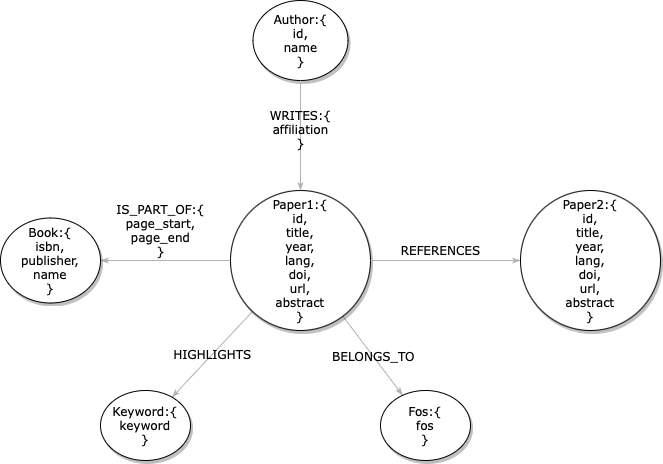
\includegraphics[width=0.9\textwidth]{Images/graph_diagram}
        \caption{Graph diagram of a Paper that references another one, it has a single Author, a Keyword, a Fos and it is part of a Book.}
        \label{fig:graph_diagram}%
    \end{center}
\end{figure}


\chapter{Commands and queries}
\label{ch:commands_and_queries_neo4j}%
The following commands and queries are written thinking principally on the way the database will be used.
We think a user with the necessity to upload or search for something in the system, will be able to do that with what we provide.
Longer and more difficult commands and queries can be written but we want to present only the ones that we find more meaningful.

We choose to use parameters instead of writing fixed values inside the queries to make the code as flexible as possible.
For this reason, the commands and queries can be also used changing the values of the parameters and obtaining the results of interest.
To execute the following code is required to run first the parameters regarding the command or query we want to perform and then the command or query itself.


\section{Commands}
\label{sec:commands}%
The following commands are provided to make possible the update of the data.
Each command can be easily modified to update parts of the database with specific features, for example, it is possible to use the queries of the next section to update the obtained nodes and their attributes.

\begin{enumerate}
    \item \textbf{Create a node, its attributes, and some relationships} \\
    The command creates a set of new nodes.
    In particular, the query aims to add a new paper to the database, whose author is already present within the system, and also set its properties.
    Here we add a new paper, set also its attributes, and create the nodes of the keywords and the fields of study of the paper if needed.
    The \verb|MERGE| command is what is used to create nodes and relationships checking also whether the new instances are already present within the database.
    This command allows us to avoid the creation of many copies of the same entity.
    The following command after adding the specified nodes creates also the relationships between them: the ones that relate the paper to its author, to its keywords, and to the specific study.

    \textbf{Parameters}
    \begin{lstlisting}[label={lst:parameters_command1neo4j}]
:param auth_id => "53f463b3dabfaee4dc8430d5";
:param auth_name => "Annabel Sebag";
:param affiliation => "53f463b3dabfaee4dc8430d5";

:param doi => "10.1145/1596685.1596829";
:param paper_id => "53e997cbb7602d9701fbcee3";
:param paper_title => "Yankee gal";
:param year => 2009;
:param lang => "en";
:param page_start => 155;
:param page_end => 155;
:param url => ["https://dx.doi.org/10.1145/1596685.1596829","https://doi.acm.org/10.1145/1596685.1596829","db/conf/siggraph/siggraph2009festival.html#Sebag09c","https://doi.org/10.1145/1596685.1596829"];
:param abstract => "This is a graduate film from the students of Supinfocom Valenciennes.";

:param k1 => "yankee gal";
:param k2 => "supinfocom valenciennes";
:param k3 => "graduatethe query aims"animation";
:param fos2 => "siggraph";
    \end{lstlisting}
    \textbf{Command}
    \begin{lstlisting}[label={lst:command1neo4j}]
MATCH (a:Author {id:$auth_id, name: $auth_name})
MERGE (new_p:Paper
        {doi:$doi,
        id:$paper_id,
        title:$paper_title,
        year:$year,
        lang:$lang,
        page_start:$page_start,
        page_end:$page_end,
        url:$url,
        abstract:$abstract})
MERGE aff = (a)-[:WRITES {affiliation:$affiliation}]->(new_p)
MERGE f1 = (new_p)-[:BELONGS_TO]->(:Fos {fos: $fos1})
MERGE f2 = (new_p)-[:BELONGS_TO]->(:Fos {fos: $fos2})
MERGE k1 = (new_p)-[:HIGHLIGHTS]->(kw1:Keyword {keyword:$k1})
MERGE k2 = (new_p)-[:HIGHLIGHTS]->(kw2:Keyword {keyword:$k2})
MERGE k3 = (new_p)-[:HIGHLIGHTS]->(kw3:Keyword {keyword:$k3})
RETURN aff, f1, f2, k1, k2, k3
    \end{lstlisting}
    \item \textbf{Create the relationship between existing nodes and set its properties} \\
    The command creates a new relationship between already existing nodes.
    In particular here is created the relationship which states that the author \verb|"James Ostell"| has written the paper titled \verb|"Grow"| when he was affiliated to organization \verb|"Federal| \verb|Institute of Technology, Switzerland"|.
    For better identification of the book and for avoiding linking all the books having the same title we could have used the identifier of the book instead of the title.
    We used \verb|MERGE| so if the relationship already exists with the specified affiliation it won't be added.

    \textbf{Parameters}
    \begin{lstlisting}[label={lst:parameters_command2neo4j}]
:param name => "James Ostell";
:param title => "Grow";
:param affiliation => "Federal Institute of Technology, Switzerland";
    \end{lstlisting}
    \textbf{Command}
    \begin{lstlisting}[label={lst:command2neo4j}]
MATCH (a:Author {name:$name}), (np:Paper {title:$title})
MERGE res = (a)-[:WRITES {affiliation:$affiliation}]->(np)
RETURN res;
    \end{lstlisting}
    \item \textbf{Set a new label for a node} \\
    We want to modify the properties of an already existing node.
    In particular, we want to add one label to a specific node.
    At first, we have new entries that are sparse data and we don’t know the exact type and source so we want to infer it, in particular, we check if they have the \verb|isbn| and in that case, we update the data, setting the nodes as books.
    We do this by controlling the papers and using the \verb|SET| keyword to update the properties, and if there are some misaligned data already in the graph this corrects that too.
    In the command, we can return the nodes in order to be sure that the information was updated correctly.
    We could do the same for the relationships, and we could also add more than one label.
    \begin{lstlisting}[label={lst:command3neo4j}]
MATCH (p:Publication)
WHERE p.isbn IS NOT NULL
SET p:Book
RETURN p;
    \end{lstlisting}
    \item \textbf{Update attributes of a relationship (analog for nodes)} \\
    The next command updates the values of the attributes of a specific relationship.
    In particular, the number of the starting and ending pages of the paper with id \verb|53e99785b7602d9701f40556| are set through the keyword \verb|SET|.
    If the user makes a mistake while inserting the properties of the relationship \verb|IS_PART_OF|, let's say the pages, the user can always modify afterwards the entries with the \verb|SET| operation.
    With the same syntax, if new properties come up or something was missed when adding nodes or relationships it is possible to create new attributes and set them to a specific value.

    \textbf{Parameters}
    \begin{lstlisting}[label={lst:parameters_command4neo4j}]
:param id => "53e99785b7602d9701f40556";
    \end{lstlisting}
    \textbf{Command}
    \begin{lstlisting}[label={lst:command4neo4j}]
MATCH (paper:Paper)-[i:IS_PART_OF]->(:Book)
WHERE paper.id = $id
SET i.page_start = 15
SET i.page_end = 33
    \end{lstlisting}
    \item \textbf{Remove attributes of a relationship (analogous for nodes)} \\
    The following commands remove some attributes from a relationship.
    In particular, we remove the attributes concerning the starting and ending numbers of pages within a book when these numbers are negative.
    We also remove these numbers when the index of the starting page is greater than the index of the ending page because it doesn't make sense to have such data.
    This can be seen as some sort of data cleaning, useful to remove incorrect data.
    \begin{lstlisting}[label={lst:command5neo4j1}]
MATCH (:Paper)-[i:IS_PART_OF]->(:Book)
WHERE i.page_start < 0
REMOVE i.page_start
    \end{lstlisting}
    \begin{lstlisting}[label={lst:command5neo4j2}]
MATCH (:Paper)-[i:IS_PART_OF]->(:Book)
WHERE i.page_end < 0
REMOVE i.page_end
    \end{lstlisting}
    \begin{lstlisting}[label={lst:command5neo4j3}]
MATCH (:Paper)-[i:IS_PART_OF]->(:Book)
WHERE NOT i.page_start IS NULL AND NOT i.page_end IS NULL AND i.page_end - i.page_start < 0
REMOVE i.page_start, i.page_end
    \end{lstlisting}
    \item \textbf{Delete a node} \\
    With the following command we delete the node \verb|Book| titled \verb|"Mathematics| \verb|and| \verb|Computers| \verb|in| \verb|Simulation"|, using the \verb|DELETE| keyword.
    Before performing the delete action, we use the \verb|DETACH| keyword that assures that all the relationships in which the node was involved are detached from the node itself in order to be able to remove it.

    \textbf{Parameters}
    \begin{lstlisting}[label={lst:parameters_command6neo4j}]
:param name => "Mathematics and Computers in Simulation";
    \end{lstlisting}
    \textbf{Command}
    \begin{lstlisting}[label={lst:command6neo4j}]
MATCH (b:Book {name:$name})
DETACH DELETE b;
    \end{lstlisting}
\end{enumerate}


\section{Queries}
\label{sec:queries}%
\begin{enumerate}
    \item \textbf{Authors who wrote a certain paper} \\
    The query returns a graph with all the authors who wrote the papers titled \verb|"CodeTalk"|.
    This is a very simple query that can be very useful in everyday searches.

    \textbf{Parameters}
    \begin{lstlisting}[label={lst:parameters_query1neo4j}]
:param title => "CodeTalk";
    \end{lstlisting}
    \textbf{Query}
    \begin{lstlisting}[label={lst:query1neo4j}]
MATCH g = (:Author)-[:WRITES]->(:Paper {title:$title})
RETURN g
    \end{lstlisting}
    \begin{figure}[H]
        \begin{center}
            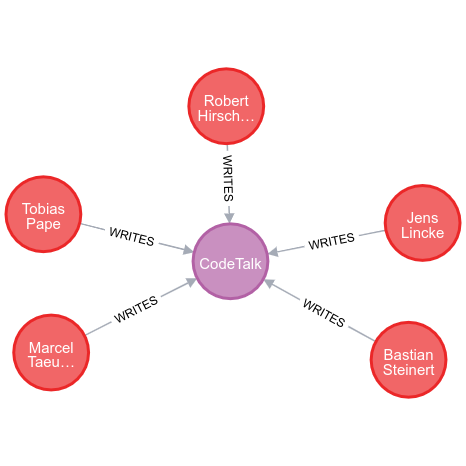
\includegraphics[trim={0 1cm 0 0}, clip, width=0.45\textwidth]{Images/query1neo4j}
            \label{fig:query1neo4j}%
        \end{center}
    \end{figure}
    \item \textbf{Previous affiliations of an author} \\
    The query returns all the organizations to whom the author \verb|"Annabel Sebag"| has been affiliated sorted by the year in which she wrote the paper with that affiliation.

    \textbf{Parameters}
    \begin{lstlisting}[label={lst:parameters_query2neo4j}]
:param name => "Annabel Sebag";
    \end{lstlisting}
    \textbf{Query}
    \begin{lstlisting}[label={lst:query2neo4j}]
MATCH (:Author {name:$name})-[r:WRITES]-(p:Paper)
WITH r.affiliation AS affiliation, p.year AS year
ORDER BY year DESC
RETURN DISTINCT affiliation, year
    \end{lstlisting}
    \begin{figure}[H]
        \begin{center}
            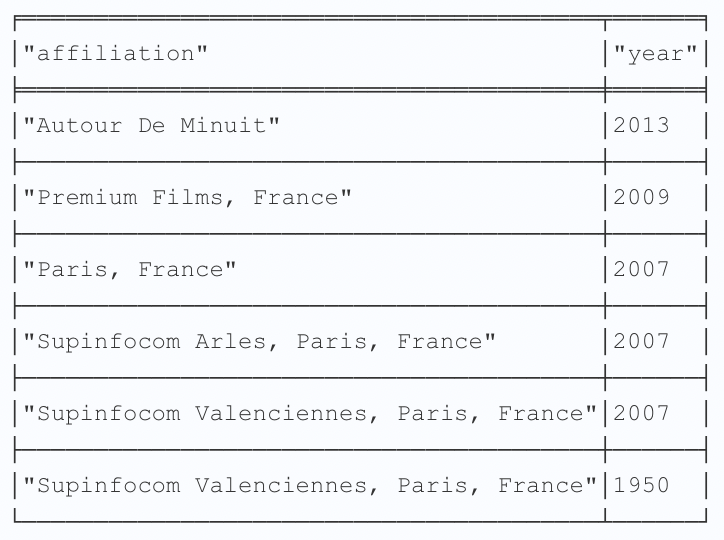
\includegraphics[width=0.45\linewidth]{Images/query2neo4j}
            \label{fig:query2neo4j}%
        \end{center}
    \end{figure}
    \item \textbf{Authors who wrote for a journal in a specific year} \\
    The query returns all the authors who wrote at least a paper for the journal named \verb|"Briefings in Bioinformatics"| in the year \verb|2005|.
    In the return statement we use the keyword \verb|DISTINCT| in order to count only once each author because we only want to know if the author wrote on that paper in the specified year, and not how many times.

    \textbf{Parameters}
    \begin{lstlisting}[label={lst:parameters_query3neo4j}]
:param name => "Briefings in Bioinformatics";
:param year => 2005;
    \end{lstlisting}
    \textbf{Query}
    \begin{lstlisting}[label={lst:query3neo4j}]
MATCH (a:Author)-[:WRITES]->(p:Paper)-[:IS_PART_OF]->(j:Journal)
WHERE p.year = $year AND j.name = $name
RETURN DISTINCT a.name AS authorName
    \end{lstlisting}
    \begin{figure}[H]
        \begin{center}
            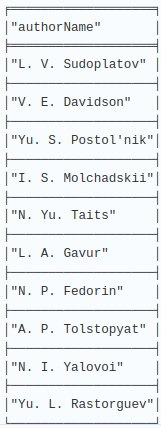
\includegraphics[width=0.45\textwidth]{Images/query3neo4j}
            \label{fig:query3neo4j}%
        \end{center}
    \end{figure}
    \item \textbf{Papers that belong to a Journal, written by authors while they were affiliated to a certain organization} \\
    The query returns the names of all the journals written by authors while they were affiliated with the organization named \verb|"Wien"|.

    In some of the queries we have seen before, we retrieved from the database the affiliations related to the authors.
    It is also interesting to see how easily we can retrieve the authors that are related to a certain affiliation, and then explore the relationships of the author in order to obtain meaningful data, useful for everyday search in the bibliography database.
    The next query is very fast because centered mostly on relationships, a natural characteristic of graphs.

    \textbf{Parameters}
    \begin{lstlisting}[label={lst:parameters_query4neo4j}]
:param affiliation => "Wien";
    \end{lstlisting}
    \textbf{Query}
    \begin{lstlisting}[label={lst:query4neo4j}]
MATCH (:Author)-[:WRITES {affiliation:$affiliation}]->(:Paper)-[:IS_PART_OF]->(b:Journal)
RETURN DISTINCT b.name as journalName;
    \end{lstlisting}
    \begin{figure}[H]
        \begin{center}
            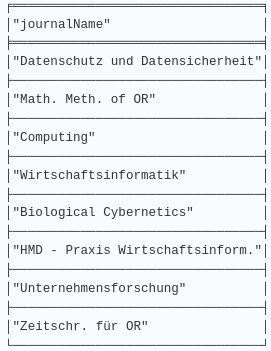
\includegraphics[width=0.45\textwidth]{Images/query4neo4j}
            \label{fig:query4neo4j}%
        \end{center}
    \end{figure}
    \item \textbf{Authors which published more papers in journals in a specific year} \\
    The query returns the five authors that published more papers in the year \verb|2000| in journals sorted by the number of papers they published.
    We use the function \verb|count()| to obtain for each author the relative number of papers and limit the output to the first five authors discovered during the search.

    \textbf{Parameters}
    \begin{lstlisting}[label={lst:parameters_query5neo4j}]
:param year => 2000;
    \end{lstlisting}
    \textbf{Query}
    \begin{lstlisting}[label={lst:query5neo4j}]
MATCH (a:Author)-[:WRITES]->(p:Paper)-[:IS_PART_OF]->(:Journal)
WHERE p.year = $year
WITH a, count(*) AS paperNum
RETURN a.name AS authorName, paperNum
ORDER BY paperNum DESC LIMIT 5;
    \end{lstlisting}
    \begin{figure}[H]
        \begin{center}
            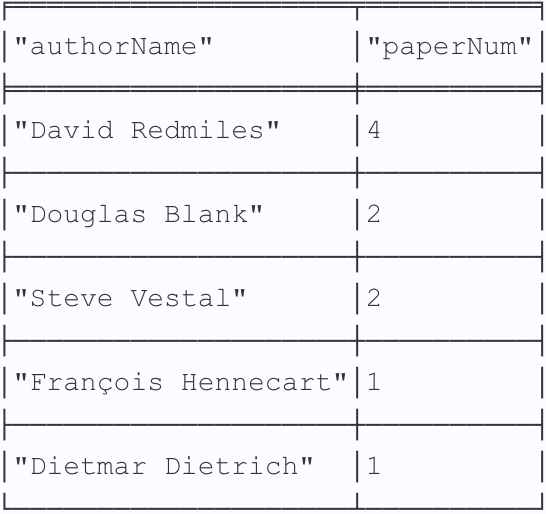
\includegraphics[width=0.45\textwidth]{Images/query5neo4j}
            \label{fig:query5neo4j}%
        \end{center}
    \end{figure}
    \item \textbf{Number of papers written in conferences by authors whose name starts with specific letters per venue} \\
    The query returns for each venue the number of papers that have been presented in a conference considering only papers that are written by authors whose name starts for \verb|"A"| or \verb|"S"|.

    \textbf{Parameters}
    \begin{lstlisting}[label={lst:parameters_query6neo4j}]
:param letter1 => "A";
:param letter2 => "S";
    \end{lstlisting}
    \textbf{Query}
    \begin{lstlisting}[label={lst:query6neo4j}]
MATCH (a:Author)-[:WRITES]->(p:Paper)-[:IS_PART_OF]->(c:Conference)
WHERE a.name STARTS WITH $letter1 OR a.name STARTS WITH $letter2
WITH c.name AS conference, c.location AS location,
     count(DISTINCT p) AS number_of_papers
RETURN DISTINCT conference, location, number_of_papers
ORDER BY number_of_papers DESC LIMIT 5;
    \end{lstlisting}
    \begin{figure}[H]
        \begin{center}
            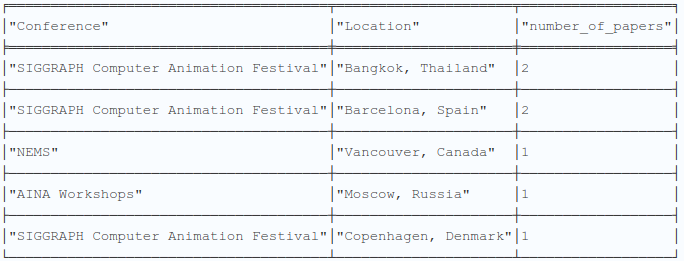
\includegraphics[width=0.9\textwidth]{Images/query6neo4j}
            \label{fig:query6neo4j}%
        \end{center}
    \end{figure}
    \item \textbf{Authors who wrote the most referenced papers which belong to publications of type book, while they were affiliated to a specific organization} \\
    The query returns the authors whose papers have been referenced the most in papers that are part of books while they were affiliated to \verb|"University of Mannheim"|.
    We also want to retrieve only authors that published at least 2 papers, so we filter furthermore the result.

    \textbf{Parameters}
    \begin{lstlisting}[label={lst:parameters_query7neo4j}]
:param affiliation => "University of Mannheim";
    \end{lstlisting}
    \textbf{Query}
    \begin{lstlisting}[label={lst:query7neo4j}]
MATCH (a:Author)-[w:WRITES]->(:Paper)<-[r:REFERENCES]-(:Paper)-[:IS_PART_OF]->(:Book)
WHERE w.affiliation = $affiliation
WITH a, count(DISTINCT r) AS totalReferences
WHERE totalReferences > 2
RETURN a.name AS authorName, totalReferences;
    \end{lstlisting}
    \begin{figure}[H]
        \begin{center}
            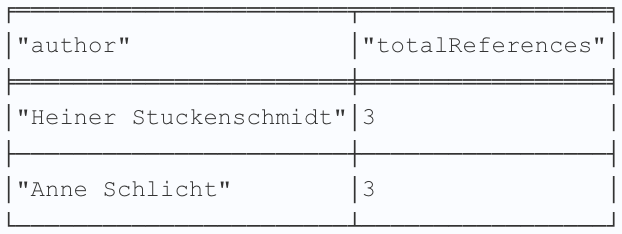
\includegraphics[width=0.45\linewidth]{Images/query7neo4j}
            \label{fig:query7neo4j}%
        \end{center}
    \end{figure}
    \item \textbf{Papers indirectly referenced by other papers at a certain distance of steps} \\
    The query returns different papers linked to each other by the relation \verb|REFERENCES| at a distance of steps between 3 and 6.
    We limit the results in order to get the output as soon as the process finds 5 rows that respect the filter of the search.
    \begin{lstlisting}[label={lst:query8neo4j1}]
MATCH (a1:Paper), (a2:Paper)
WHERE id(a1) <> id(a2) AND (EXISTS {MATCH (a1)-[:REFERENCES*3..6]->(a2)})
RETURN DISTINCT a1.title AS firstPaper, a2.title AS secondPaper
LIMIT 5;
    \end{lstlisting}
    \begin{figure}[H]
        \begin{center}
            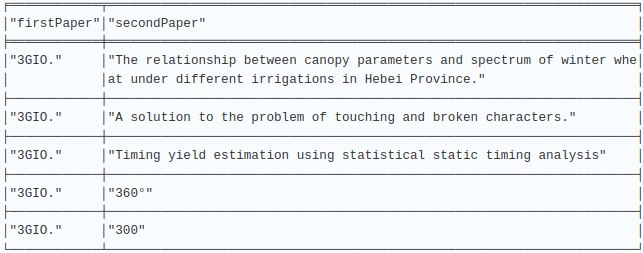
\includegraphics[width=0.9\textwidth]{Images/query8neo4j1}
            \label{fig:query8neo4j}%
        \end{center}
    \end{figure}
    The performance is not optimal and using the \verb|PROFILE| command in the same query we can see how the search is actually made in the graph using this specific interrogation on the database.
    \begin{lstlisting}[label={lst:profile_query8neo4j1}]
PROFILE
MATCH (a1:Paper), (a2:Paper)
WHERE id(a1) <> id(a2) AND (EXISTS {MATCH (a1)-[:REFERENCES*3..6]->(a2)})
RETURN DISTINCT a1.title AS firstPaper, a2.title AS secondPaper LIMIT 5;
    \end{lstlisting}
    \begin{figure}[H]
        \begin{center}
            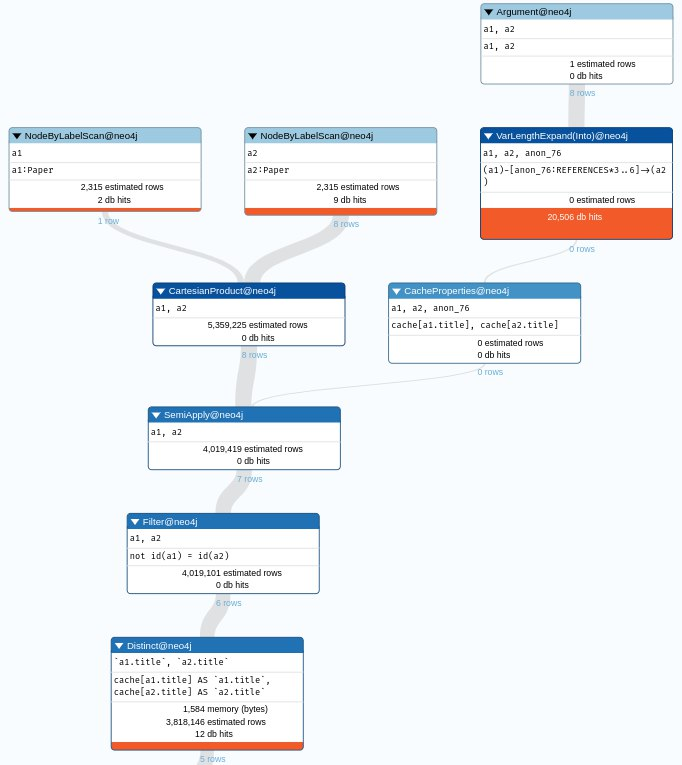
\includegraphics[width=0.9\textwidth]{Images/profile_query8neo4j1}
            \label{fig:profile_query8neo4j1}%
        \end{center}
    \end{figure}
    We can notice that the execution of the query is done in parallel trying on one side to perform the \verb|MATCH| of the two papers separately and on the other side to find the relationships between the two papers given by \verb|REFERENCES| from 3 to 6 steps away.
    The two results of the search are then merged together. \\
    In this process, we estimated a lot of rows and wasted time, by doing the controls individually.
    \begin{figure}[H]
        \begin{center}
            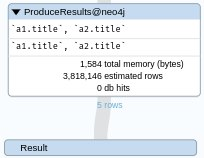
\includegraphics[width=0.45\textwidth]{Images/result_query8neo4j1}
            \label{fig:result_query8neo4j1}%
        \end{center}
    \end{figure}
    To make the query more efficient we can bring the filtering of the data a step ahead, so we can check directly in the \verb|MATCH| command for the relationships between the papers.
    \begin{lstlisting}[label={lst:query8neo4j2}]
MATCH (a1:Paper)-[:REFERENCES*3..6]->(a2:Paper)
WHERE id(a1) <> id(a2)
RETURN DISTINCT a1.title AS firstPaper, a2.title AS secondPaper
LIMIT 5;
    \end{lstlisting}
    We notice that the results can be different from the precedent approach, due to the use of \verb|LIMIT| that stops the research as soon as it gets the 5 results of interest and in this case, the search is done differently so the outputs are not the same.
    \begin{figure}[H]
        \begin{center}
            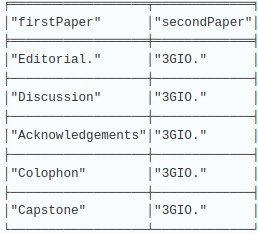
\includegraphics[width=0.45\textwidth]{Images/query8neo4j2}
            \label{fig:query8neo4j2}%
        \end{center}
    \end{figure}
    Using this version of the query, we have that the search is more linear because, in \verb|MATCH|, we don't look for the papers separately but once matched a \verb|Paper| we search for its recursive \verb|REFERENCES| relationships and match at once the two papers and their connections.
    This approach is fast and improves efficiency.
    \begin{figure}[H]
        \begin{center}
            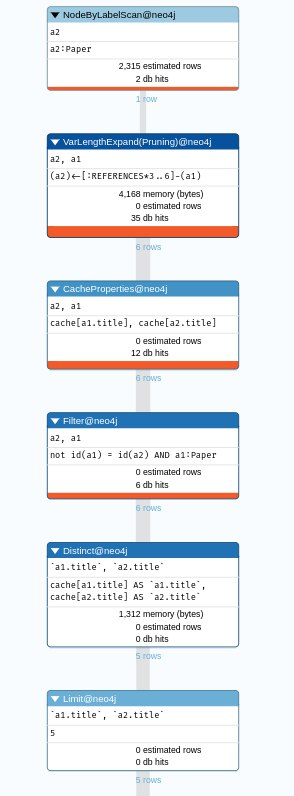
\includegraphics[width=0.45\textwidth]{Images/profile_query8neo4j2}
            \label{fig:profile_query8neo4j2}%
        \end{center}
    \end{figure}
    We can see that reaching the result the command required more memory, but we didn't estimate useless rows of data, extracting only what we are interested in without an extended search on the graph.
    \begin{figure}[H]
        \begin{center}
            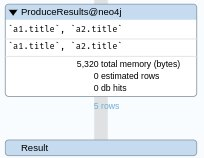
\includegraphics[width=0.45\textwidth]{Images/result_query8neo4j2}
            \label{fig:result_query8neo4j2}%
        \end{center}
    \end{figure}
    Alternatively, we can tackle this search from another point of view.
    We can use a query based precisely on the steps we are interested in, making the query more explicit and getting other results, because in the recursive form the process could stop before reaching this exact amount of steps, especially using the \verb|LIMIT| keyword.
    \begin{lstlisting}[label={lst:query8neo4j3}]
MATCH (a1:Paper)-[:REFERENCES]->(a2:Paper)-[:REFERENCES]->(a3:Paper)-[:REFERENCES]->(a4:Paper)-[:REFERENCES]->(a5:Paper)-[:REFERENCES]->(a6:Paper)
WHERE id(a1) <> id(a2) AND id(a2) <> id(a3) AND id(a3) <> id(a4) AND id(a4) <> id(a5) AND id(a5) <> id(a6)
RETURN DISTINCT a1.title AS firstPaper, a6.title AS secondPaper
LIMIT 5;
    \end{lstlisting}
    \begin{figure}[H]
        \begin{center}
            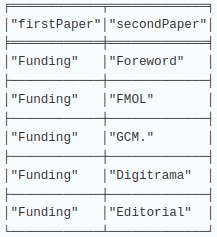
\includegraphics[width=0.45\textwidth]{Images/query8neo4j3}
            \label{fig:query8neo4j3}%
        \end{center}
    \end{figure}
    \item \textbf{Best collaborator of all times for each author in terms of papers written in journals} \\
    The following query allows the researcher to understand each author who is the best collaborator of all time considering their collaborations in journals.
    In the result, we can sometimes see symmetry in the data, if an author has another as the best collaborator and vice versa.

    Firstly we do a \verb|MATCH| imposing our constraints.
    Secondly, we group by authors and co-authors counting for each couple how many papers were published in journals they wrote together, and we order the table by this number in descending order.
    On the next \verb|WITH| clause for each author we extract only the best collaborator, namely the one with whom he wrote more papers in journals.

    \textbf{Query}
    \begin{lstlisting}[label={lst:query9neo4j}]
MATCH (a:Author)-[:WRITES]->(p:Paper)<-[:WRITES]-(ca:Author), (p)-[:IS_PART_OF]->(:Journal)
WITH DISTINCT a, ca, count(DISTINCT p) AS cnt ORDER BY cnt DESC
WITH DISTINCT a, collect(ca.name) AS colabs, collect(cnt) AS cnts
RETURN a.name AS author, colabs[0] AS bestCollaborator, cnts[0] AS numberOfPapers LIMIT 5
    \end{lstlisting}
    \begin{figure}[H]
        \begin{center}
            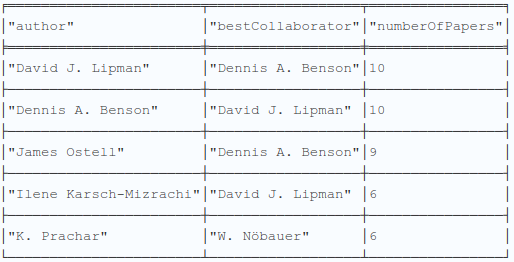
\includegraphics[width=0.9\textwidth]{Images/query9neo4j}
            \label{fig:query9neo4j}%
        \end{center}
    \end{figure}
    \item \textbf{Papers which are at the base of a given field of study} \\
    The query returns the papers which are at the base of a given field of study.
    To be the base for a field of study means to not reference directly or indirectly other papers of that field of study.
    With this query, we retrieve the papers that are probably at the base of some field of study because an upper bound of 7 is chosen to check the indirect references. \\
    A variant of this query can be to retrieve the authors who wrote the base papers of a field of study, so the authors are the ``founders'' of that field.
    The query is more meaningful if run on a very large set of data.
    \textbf{Parameters}
    \begin{lstlisting}[label={lst:parameters_query10neo4j}]
:param fos => "Statistics";
    \end{lstlisting}
    \textbf{Query}
    \begin{lstlisting}[label={lst:query10neo4j}]
MATCH (founder:Paper)-[:BELONGS_TO]->(fos:Fos{fos:$fos})<-[:BELONGS_TO]-(p:Paper)
WHERE id(founder) <> id(p)
WITH collect(p) AS test, founder, fos
WHERE all(p IN test WHERE NOT EXISTS((founder)-[:REFERENCES*7]->(p)))
RETURN fos AS field, collect(DISTINCT founder.title) AS founderPapers
    \end{lstlisting}
    \begin{figure}[H]
        \begin{center}
            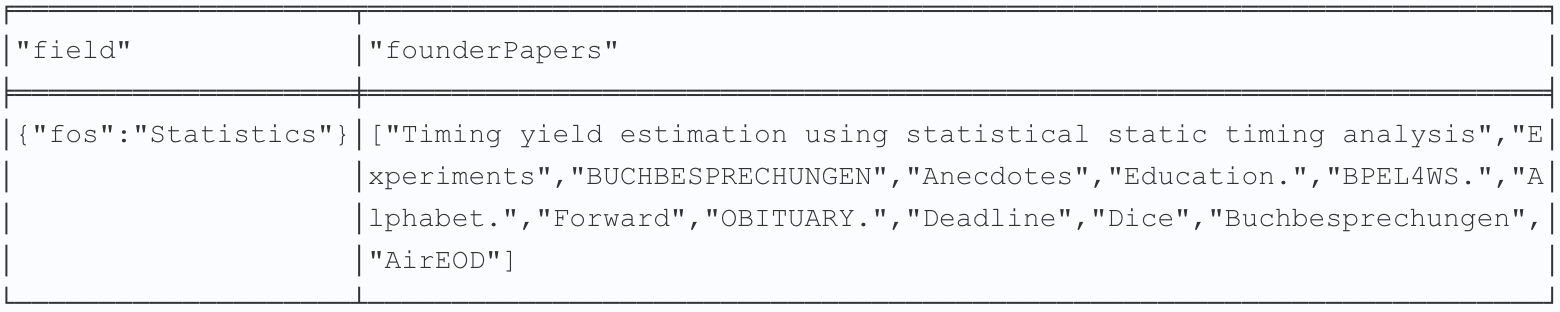
\includegraphics[width=0.9\linewidth]{Images/query10neo4j}
            \label{fig:query10neo4j}%
        \end{center}
    \end{figure}
    \item \textbf{Total pages written by the authors of an organization within a journal} \\
    The query returns the total number of pages written by authors affiliated with the organization \verb|"Federal Institute of Technology, Switzerland"| within journals.
    The function \verb|avg()| can be used to compute the average of the pages written by an author in the papers.

    \textbf{Parameters}
    \begin{lstlisting}[label={lst:parameters_query11neo4j}]
:param affiliation=>"Federal Institute of Technology, Switzerland";
    \end{lstlisting}
    \textbf{Query}
    \begin{lstlisting}[label={lst:query11neo4j}]
MATCH (a:Author)-[w:WRITES {affiliation:$affiliation}]->(p:Paper)-[i:IS_PART_OF]->(j:Journal)
WHERE i.page_start IS NOT NULL AND i.page_end IS NOT NULL
WITH a, sum(i.page_end - i.page_start) AS num_pag
ORDER BY num_pag DESC
RETURN a AS Author, num_pag;
    \end{lstlisting}
    \begin{figure}[H]
        \begin{center}
            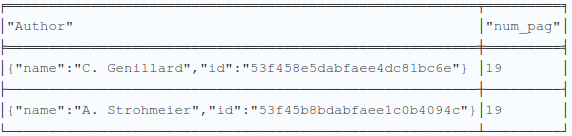
\includegraphics[width=0.9\textwidth]{Images/query11neo4j}
            \label{fig:query11neo4j}%
        \end{center}
    \end{figure}
    \item \textbf{Organizations which have published their own more papers within a specific journal with associated fields of study} \\
    The query returns the organizations which have exclusively written more papers, which means that the authors of the papers have all the same affiliation on \verb|"Commun . ACM"|.
    The query provides the fields of study on which the considered papers were focused on.

    \textbf{Parameters}
    \begin{lstlisting}[label={lst:parameters_query12neo4j}]
:param journalTitle => "Commun. ACM";
    \end{lstlisting}
    \textbf{Query}
    \begin{lstlisting}[label={lst:query12neo4j}]
MATCH (a1:Author)-[w1:WRITES]->(p1:Paper)-[:IS_PART_OF]->(j:Journal {name:$journalTitle}), (p1:Paper)-[:BELONGS_TO]->(fos:Fos), (a2:Author)-[w2:WRITES]-(p1:Paper)
WHERE a1 <> a2 AND w1.affiliation IS NOT NULL
WITH w1.affiliation AS affiliation, collect(DISTINCT fos) AS fieldsOfStudy, collect(DISTINCT w2.affiliation) AS others, count(DISTINCT p1) AS numberOfPapers
WHERE ALL(organization IN others WHERE affiliation=organization)
WITH affiliation, fieldsOfStudy, numberOfPapers
ORDER BY numberOfPapers DESC
RETURN affiliation, fieldsOfStudy, numberOfPapers
LIMIT 2
    \end{lstlisting}
    \begin{figure}[H]
        \begin{center}
            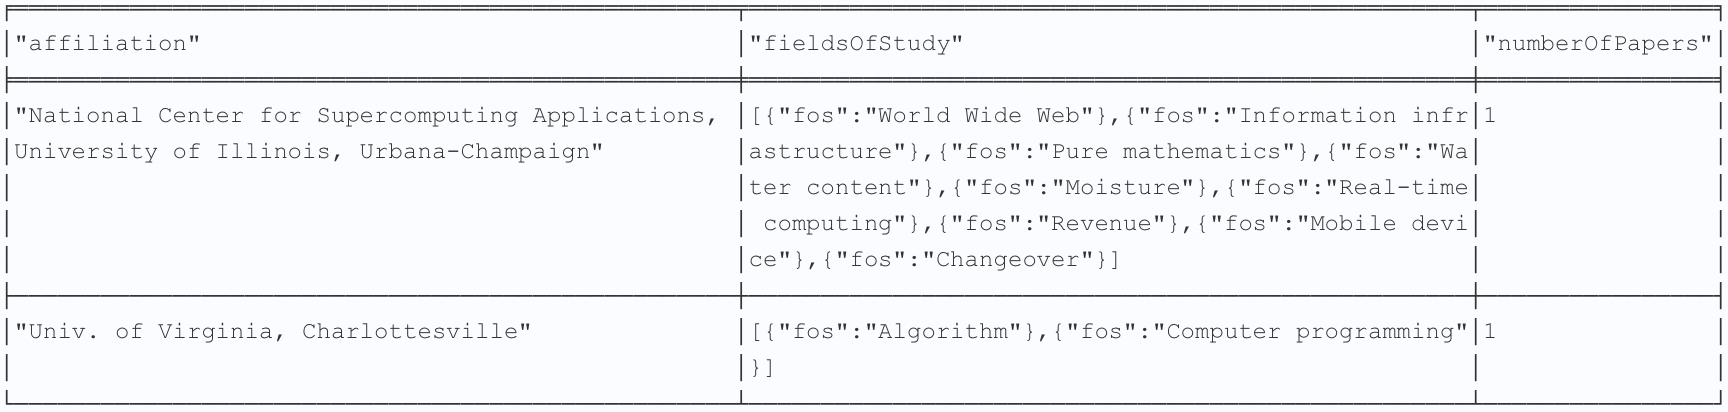
\includegraphics[width=0.9\linewidth]{Images/query12neo4j}
            \label{fig:query12neo4j}%
        \end{center}
    \end{figure}
    \item \textbf{Recommended books given one book} \\
    The query returns the book considered the nearest to the one given as a parameter.
    The similarity between books is evaluated in terms of the number of keywords associated with the papers linked to the books.
    In addition, fields of study which are common to the two books are shown.
    \begin{lstlisting}[label={lst:parameters_query13neo4j}]
:param title => "RoboCup 2009";
    \end{lstlisting}
    \textbf{Query}
    \begin{lstlisting}[label={lst:query13neo4j}]
MATCH (p1:Paper)-[:IS_PART_OF]->(b1:Book),
(p1:Paper)-[:BELONGS_TO]->(fos1:Fos)<-[:BELONGS_TO]-(p2:Paper),
(p1)-[:HIGHLIGHTS]->(k1:Keyword)<-[:HIGHLIGHTS]-(p2),
(p2:Paper)-[:IS_PART_OF]->(b2:Book)
WHERE b1 <> b2 AND p1 <> p2 AND b1.name = $title
WITH b1, b2, collect(DISTINCT fos1) AS fos, count(DISTINCT k1) AS score
ORDER BY score DESC
RETURN b2.name AS relatedBook, fos, score
LIMIT 3;
    \end{lstlisting}
    \begin{figure}[H]
        \begin{center}
            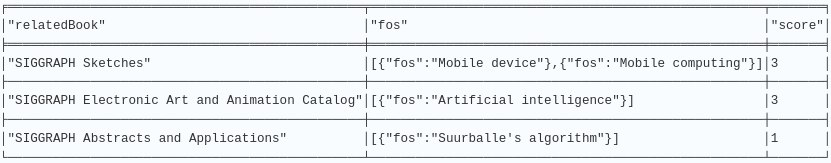
\includegraphics[width=0.9\textwidth]{Images/query13neo4j}
            \label{fig:query13neo4j}%
        \end{center}
    \end{figure}
    \item \textbf{Possible new interesting collaborations between authors in the same fields of study} \\
    The query returns the new possible interesting collaborations, by which we mean the couple of authors who haven't written a paper together but have written many times with common authors and wrote about similar topics, so they are involved in the same fields of study.

    \textbf{Parameters}
    \begin{lstlisting}[label={lst:parameters_query14neo4j}]
:param minimum_collabs =>1;
    \end{lstlisting}
    \textbf{Query}
    \begin{lstlisting}[label={lst:query14neo4j}]
MATCH
(a1:Author)-[w1:WRITES]->(p1:Paper)<-[w2:WRITES]-(a2:Author),
(a2:Author)-[w3:WRITES]->(p2:Paper)<-[w4:WRITES]-(a3:Author),
(a1)-[:WRITES]->(p3:Paper)-[:BELONGS_TO]->(f1:Fos)<-[:BELONGS_TO]-(p4:Paper)<-[:WRITES]-(a3)
WHERE NOT EXISTS ((a1)-[:WRITES]->(:Paper)<-[:WRITES]-(a3)) AND a1 <> a3 AND a1 <> a2 AND a2 <> a3
WITH a1, a3, collect(DISTINCT f1.fos) AS fields, count(DISTINCT f1) AS common_fields, count(DISTINCT p1) AS common_collabs1, count(DISTINCT p2) AS common_collabs2
WHERE common_collabs1 > $minimum_collabs AND common_collabs2 > $minimum_collabs
WITH a1, a3, fields, common_fields, common_collabs1 + common_collabs2 AS common_collabs
ORDER BY common_fields DESC, common_collabs DESC
RETURN DISTINCT a1.name as Author1, a3.name as Author2, fields, common_collabs, common_fields
LIMIT 5
    \end{lstlisting}
    \begin{figure}[H]
        \begin{center}
            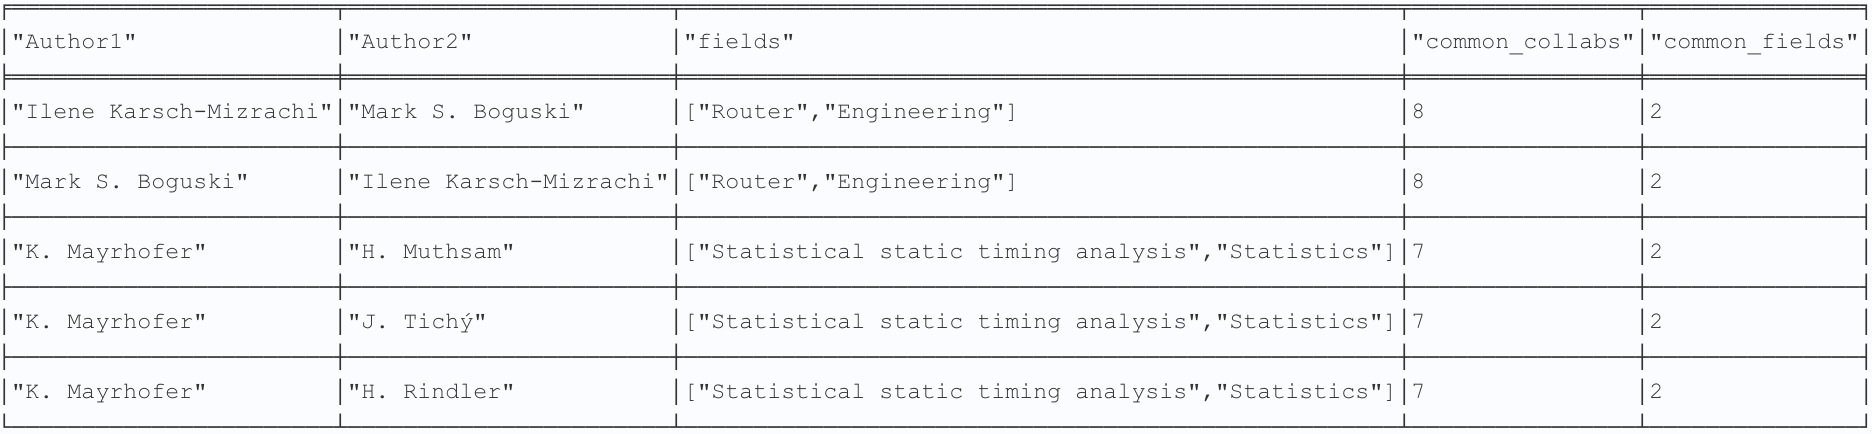
\includegraphics[width=0.9\textwidth]{Images/query14neo4j}
            \label{fig:query14neo4j}%
        \end{center}
    \end{figure}
    \item \textbf{Shortest connection between two papers with no common field of study} \\
    With this query, we want to find what is the shortest path, by navigating the references, between two papers that do not have any field of study in common.
    Firstly we bound the papers node and the associated field of studies to variables \verb|p1/p2| and \verb|fos1/fos2| respectively and we impose that \verb|p1| and \verb|p2| must be different.
    Secondly, we collect the fields of study associated with each paper and put a condition stating that the intersection of these two collection must be zero.
    Finally, we call the \verb|shortestPath| function and impose all the conditions on the path to be found;
    we put an upper bound of 7 to the length of the path to avoid searching too deep in the graph and limited the search to the first valid path found using the clause \verb|WITH sp LIMIT 1|, where \verb|sp| refers to the result of the call to the \verb|shortestPath| function.

    \textbf{Parameters}
    \begin{lstlisting}[label={lst:parameters_query15neo4j}]
:param fos1 => "Irrigation";
:param fos2 => "Artificial intelligence";
    \end{lstlisting}
    \textbf{Query}
    \begin{lstlisting}[label={lst:query15neo4j}]
MATCH (fos1:Fos) <-[:BELONGS_TO]- (p1:Paper) -[:BELONGS_TO]-> (:Fos {fos:$fos1}),
      (fos2:Fos) <-[:BELONGS_TO]- (p2:Paper) -[:BELONGS_TO]-> (:Fos {fos:$fos2})
WHERE p1 <> p2
WITH p1, collect(DISTINCT fos1) AS foss1, p2, collect(DISTINCT fos2) AS foss2
WHERE all(f IN foss1 WHERE NOT f IN foss2)
MATCH sp = shortestPath((p1)-[:REFERENCES*..7]->(p2))
WHERE length(sp) > 1
RETURN sp LIMIT 1;
    \end{lstlisting}
    Below we can see the result of the query run with the aforementioned parameters.
    \begin{figure}[H]
        \begin{center}
            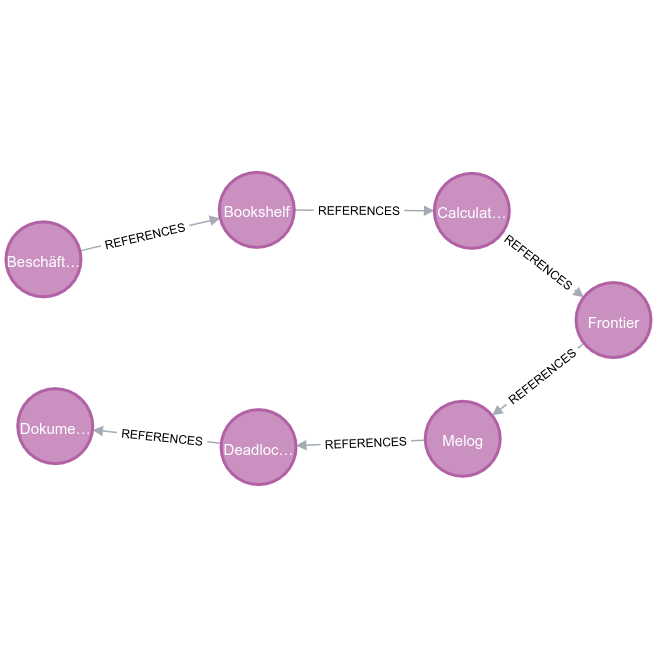
\includegraphics[trim={0 6cm 0 6cm}, clip, width=0.9\textwidth]{Images/query15neo4j}
            \label{fig:query15neo4j}%
        \end{center}
    \end{figure}
\end{enumerate}
